\section{Related Work} \label{p2background}

\begin{figure}
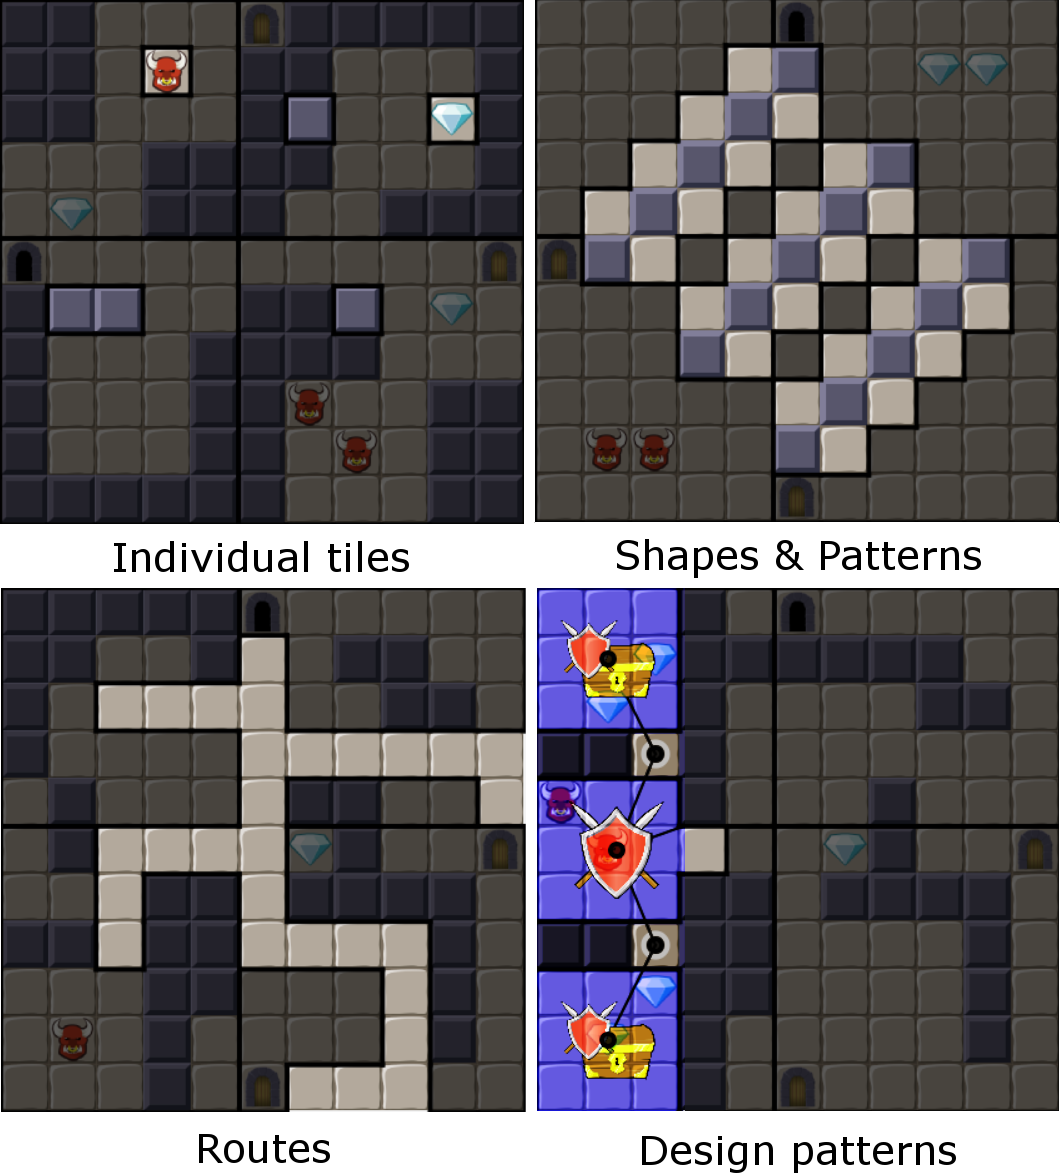
\includegraphics[scale=0.16]{Figures/figure-possible-zones}
\caption{Different uses and possibilities that the designers can have for locking the tiles in the Room, in order to, preserve their manual changes and diverse objectives}
\label{p2fig:possible-zones}
\end{figure}


Aesthetic criteria was specified by previous research as a key feature while evaluating content, as it leads to the generation of more customized content in the eyes of the human designer, whose aesthetic vision on the content is preserved~\cite{Liapis2012AdaptingCreation,Hastings2009GalacticGame,Machwe2006IntegratingInvestigation}.

%\emph{Tanagra}~\cite{Tanagra2011} is used to develop 2D platform levels. The user can place different tiles, and is able to select content, which they want to keep, while Tanagra generates content around them. 

%Aesthetic criteria has been appointed by previous research as a key feature while evaluating content, as it leads to the generation of more customized content to the eyes of the human designer, whose aesthetic vision on the content is preserved \cite{Liapis2012AdaptingCreation,Hastings2009GalacticGame,Machwe2006IntegratingInvestigation}.

Interactive evolutionary approaches incorporate human evaluation by allowing the user to select, either implicitly or explicitly, the parents of the next generation of procedurally generated individuals. In~\citet{Zhang2015DrawCompileEvolve:Creations} system allows users to draw simple primitive shapes to seed an evolutionary algorithm and train a neural network with their aesthetic vision. In Galactic Arms Race~\cite{Hastings2009GalacticGame} players preferences on the evolved weapons is implicitly deducted from the amount time they actively select those weapons during the gameplay.

\citet{Liapis2012AdaptingCreation}, incorporated visual aesthetics as an evaluation of their generated spaceships by calculating different aesthetic concepts: symmetry along axes, weight distribution or design simplicity. Moreover, ~\citet{Mario2016ACM} generated levels for Mario using symmetry as objective function, which based on their user study, were as visually pleasing as the ones created by human designers and even more than other similar approaches. 

%\citet{Liapis2012AdaptingCreation}, incorporated visual aesthetics as an evaluation of their generated spaceships by calculating different aesthetic concepts: symmetry along axes, weight distribution or design simplicity. These were computed to produce the aesthetic fitness of a spaceship, letting the user select their preferred spaceship to adjust the weight of the different aesthetic features in the fitness calculation.


%\begin{itemize}
%  \item EDDY previous versions
%  \item Previous approaches to evaluate aesthetic criteria of the designer
%  \begin{itemize}
%  	\item Aesthetic criteria was seen as visually pleasing for the designer but that does not mean that it is the idea that the user had. For mixed-initiative the way to evaluate aesthetic criteria usually was by allowing the user to select the options that he liked the most  Show examples of Mario level generator and such.
%    \item To preserve Aesthetic criteria other authors have allow the user to initiate the evolutionary algorithm with an example (initial seed) and from there, allow the evolutionary algorithm to produce suggestions based on this.
%  \end{itemize}
%\end{itemize}

%The work presented in this paper is an extension to the ongoing research of EDD \cite{Baldwin2017TowardsGeneration} and addresses the issue of preserving manual changes to the level and the impact of visual aesthetic criteria when designing dungeons.

\subsection{The Evolutionary Dungeon Designer}

EDD is a mixed-initiative authoring tool for generating dungeon rooms using a feasible-infeasible two population (fi-2pop) evolutionary approach, which is interactively evaluated and edited by a designer. The current version of EDD consists of six different building blocks that represent floors, walls, enemies, treasures, doors and entrances. This can be used by the user to brush paint and compose a NxM size room which, at its minimum, must hold one of each tile. Both the tiles and the finished room can be seen in Figure~\ref{p2fig:eddy-map}a) and b).

EDD takes the work presented in The Evolutionary World Designer~\cite{Font2016ConstrainedAlgorithms} one step further, by procedurally generating rooms and their specific content. EDD's EA follows the approach of~\citet{Liapis2012AdaptingCreation} using the evaluation of the user to change the internal evaluation and configuration of the system. Its fitness evaluation is driven by the use of game design micro- and meso- patterns, as shown in Figure \ref{p2fig:eddy-map} c) and d). A detailed description of EDD's pattern-based fitness, genetic algorithm and mixed-initiative approach can be found in \cite{Baldwin2017Mixed-initiativePatterns} and \cite{Baldwin2017TowardsGeneration}.